\documentclass[11pt]{beamer}

\usepackage[T1]{fontenc}
\usepackage[utf8x]{inputenc}
\usepackage[frenchb]{babel}
\usepackage{amsmath}
\usepackage{lmodern}
\usepackage{xcolor}
\usepackage{graphicx}
\usepackage{pstricks}

% \usepackage{lmodern}

% \usepackage[noframe]{showframe}


\usetheme{Singapore}
% \useoutertheme{smoothbars}
% \useinnertheme[shadow=true]{rounded}
% \usecolortheme{orchid}
% \usecolortheme{whale}


\setbeamertemplate{navigation symbols}{}

\definecolor{cloneBlue}{rgb}{0.2,0.2,0.698}


\newenvironment{changemargin}[2]{%
  \begin{list}{}{%
    \setlength{\topsep}{0pt}%
    \setlength{\leftmargin}{#1}%
    \setlength{\rightmargin}{#2}%
    \setlength{\listparindent}{\parindent}%
    \setlength{\itemindent}{\parindent}%
    \setlength{\parsep}{\parskip}%
  }%
  \item[]}{\end{list}} 

\newenvironment{noitemize}
{\begin{list}{}{%
\setlength{\labelwidth}{0em}% largeur de la boite englobant l'étiquette
\setlength{\labelsep}{2pt}% espace entre l'entrée de l'item et l'étiquette
\setlength{\leftmargin}{0pt}% marge de gauche
\renewcommand{\makelabel}{\small\color{cloneBlue}{\textbullet}}}}%
{\end{list}}

\newenvironment{minusitemize}
{\begin{list}{}{%
\setlength{\labelwidth}{0em}% largeur de la boite englobant l'étiquette
\setlength{\labelsep}{2pt}% espace entre l'entrée de l'item et l'étiquette
\setlength{\leftmargin}{-15pt}% marge de gauche
\renewcommand{\makelabel}{\small\color{cloneBlue}{\textbullet}}}}%
{\end{list}}


\setbeamersize{text margin left=0.75cm}
\setbeamersize{text margin right=0.75cm}


\author{Yann Boniface, Alain Dutech, Nicolas Rougier, Matthieu Zimmer}
\title{Exploration de la notion de méta-apprentissage}
\subtitle[\ldots]{Dans quelle mesure un système apprenant peut « prendre conscience » de ses performances et altérer son comportement ?}
\institute{Loria}
\date{\today}
\logo{
\includegraphics[height=6mm]{logo.png}}

\begin{document}

\maketitle



\begin{frame}
 \frametitle{Inspiration : Conscience et méta-représentations}
 \framesubtitle{Articles}
 
 \begin{itemize}
  \item Consciousness and metarepresentation : A computational sketch
  \newline [ Alex Cleeremans, Bert Timmermans, Antoine Pasquali ]
  \item Know thyself : Metacognitive networks and mesures of consciousness
  \newline [ Antoine Pasquali, Bert Timmermans, Alex Cleeremans ]
 \end{itemize}
\end{frame}



\begin{frame}
  \begin{center}{\Large Plan }\end{center}
  \tableofcontents[hideallsubsections]
\end{frame}


\section{Dupliquer le premier réseau}

\begin{frame}
  \frametitle{La base de départ / Rappel}
  \begin{center}
    \begin{pspicture}(0,5)
      \rput[B](0,0){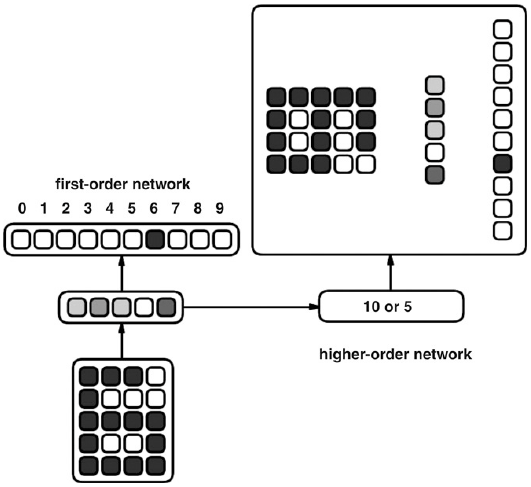
\includegraphics[height=150px]{../cleeremans_2007/digit_reco/digit_reco.png}}
      \rput[B](3,0.5){\tiny{Consciousness and metarepresentation : A computational sketch}}
    \end{pspicture}
  \end{center}

  \begin{center}
    \begin{tabular}{lr}
    \begin{minipage}{150px}
      
      \footnotesize\begin{minusitemize}
      \item 20 entrées (représentant les chiffres)
      \item le premier réseau discrime les 10 chiffres
      \item winner-take-all sur les sorties
      \end{minusitemize}

      \end{minipage}
      &
      \begin{minipage}{170px}
      \footnotesize\begin{noitemize}
      \item la couche cachée du premier réseau sert d'entrée au second
      \item le second réseau apprend à dupliquer toutes les couches du premier
      \end{noitemize}
      
    \end{minipage}
    \end{tabular}
  \end{center}
  
\end{frame}

\begin{frame}
  \frametitle{Résultat sur la base d'entrée de l'article}
  \begin{center}
  \begin{tabular}{cc}
  \hspace*{-1cm}
   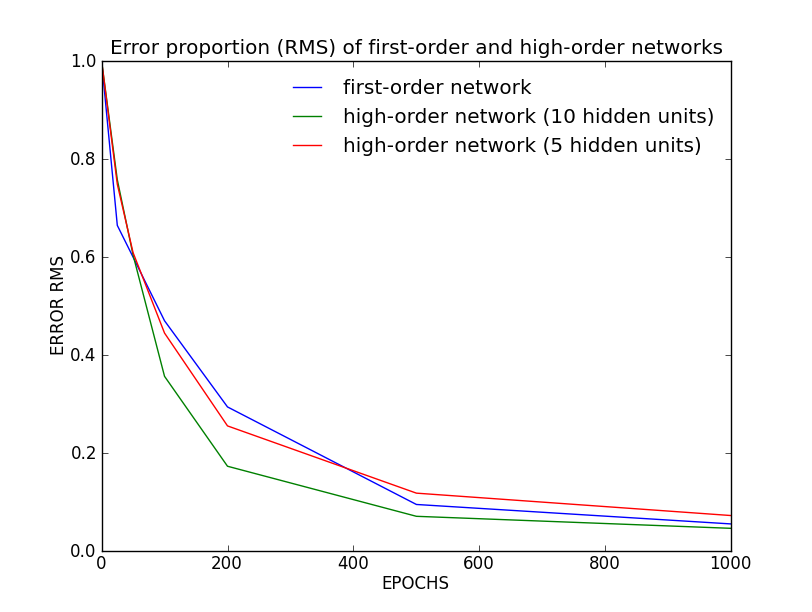
\includegraphics[width=185px]{../cleeremans_2007/digit_reco/rms.png}
   &
   \hspace*{-0.5cm}
   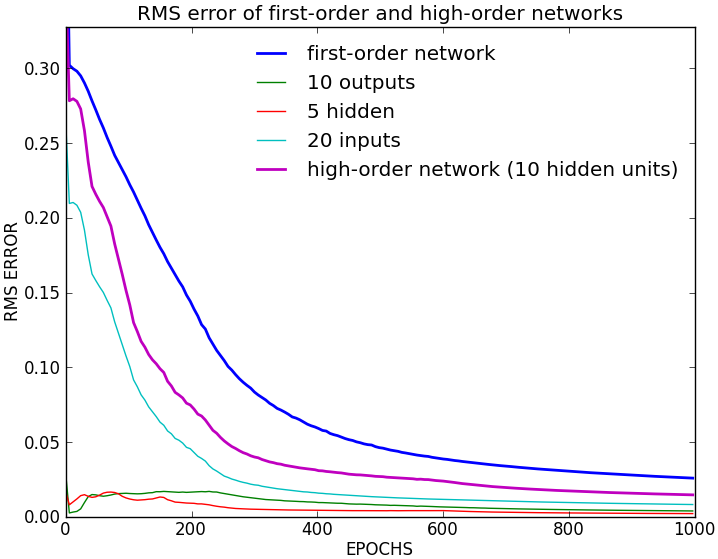
\includegraphics[width=170px]{../cleeremans_2007/digit_reco/rms_ffa.png}
  \end{tabular}
  \end{center}

\begin{itemize}
 \item la couche cachée et la couche de sortie ne posent aucun problèmes d'apprentissage
 \item les performances du second réseau dépendent principalement de sa capacité à reproduire les entrées
\end{itemize}
\end{frame}


\begin{frame}
  \frametitle{Dans la couche cachée du FoN : les entrées du SoN}
  \begin{center}
   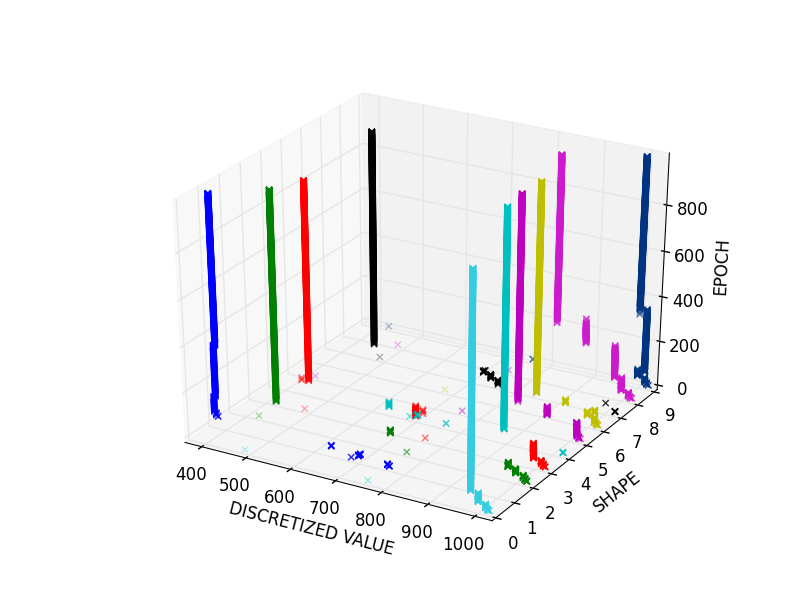
\includegraphics[width=185px]{../cleeremans_2007/digit_reco/discretize_cloud.png}
  \end{center}

\begin{itemize}
 \item stabilisation très rapidement (autour de la 50\up{ième} époque en moyenne)
 \item entrées peu variables et stable favorisant son apprentissage
\end{itemize}
\end{frame}



\begin{frame}
  \frametitle{Passage à niveau}
  \begin{center}
  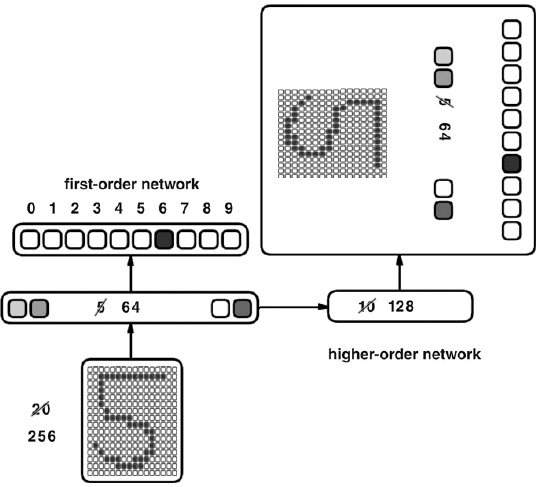
\includegraphics[height=150px]{../cleeremans_2007/digit_reco/schema_handwritten.png}
  \end{center}

  \begin{center}
  \begin{tabular}{lr}
  \begin{minipage}{150px}
    
    \footnotesize\begin{minusitemize}
     \item chiffres manuscrits sur 256 neurones d'entrées
     \item Le premier réseau discrime \textbf{1600 chiffres}
     \item Winner-take-all sur les sorties
    \end{minusitemize}

    \end{minipage}
    &
    \begin{minipage}{170px}
    \footnotesize\begin{noitemize}
     \item la couche cachée du premier réseau sert d'entrée au second
     \item le second réseau apprend à dupliquer toutes les couches du premier
    \end{noitemize}
    
    \end{minipage}
  \end{tabular}

  \end{center}
  
\end{frame}


\begin{frame}
  \frametitle{Résultats}
  \begin{center}
  \begin{tabular}{cc}
  \hspace*{-1cm}
   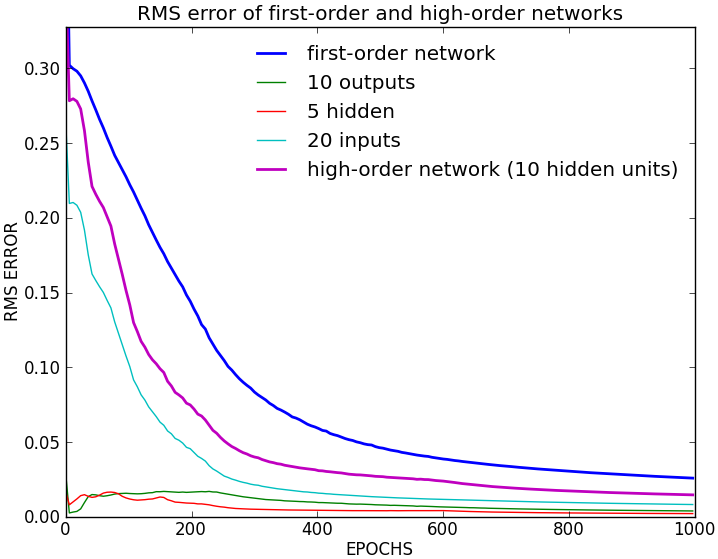
\includegraphics[width=175px]{../cleeremans_2007/digit_reco/rms_ffa.png}
   &
   \hspace*{-0.5cm}
   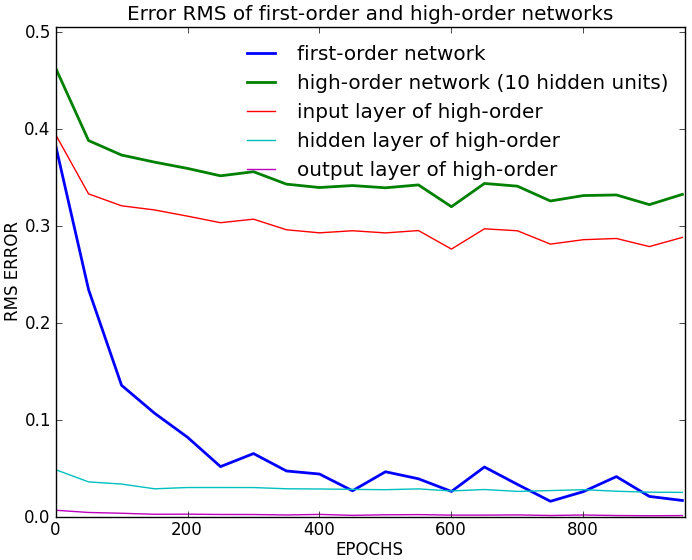
\includegraphics[width=170px]{../cleeremans_2007/digit_reco/rms_handwritten_ffa.png}
  \end{tabular}
  \end{center}

\begin{itemize}
 \item la couche cachée et la couche de sortie s'apprennent toujours bien
 \item il n'arrive plus à dupliquer les entrées
 \item ça fonctionne dans l'article car il n'y a que 10 entrées différentes
\end{itemize}
\end{frame}


\begin{frame}
  \frametitle{Dans la couche cachée du FoN : les entrées du SoN}
  \begin{center}
   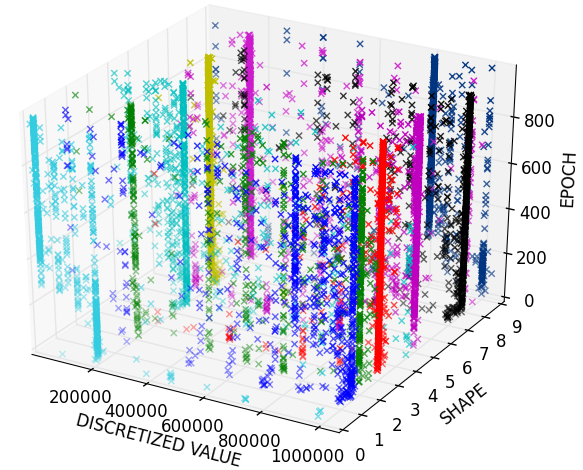
\includegraphics[height=160px]{../cleeremans_2007/digit_reco/discretize_minhand.png}
  \end{center}

\begin{itemize}
 \item il existe différentes valeurs de la couche cachée, représentant le même nombre
 \item une même valeur discrétisée peut correspondre à  plusieurs couleurs
\end{itemize}
\end{frame}


\begin{frame}
  \frametitle{Représentation interne}
  
    \begin{center}
  \begin{tabular}{cc}
  \hspace*{-1cm}
   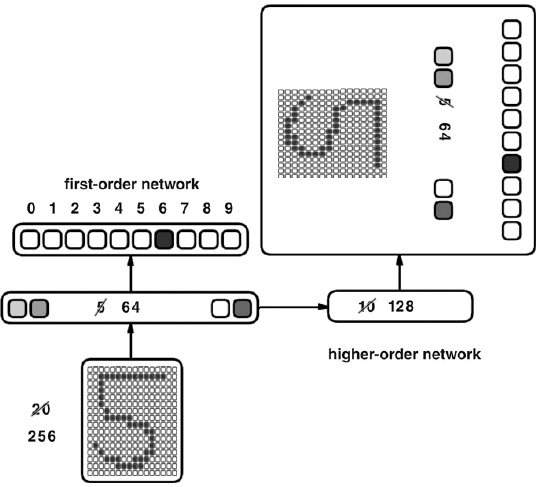
\includegraphics[width=130px]{../cleeremans_2007/digit_reco/schema_handwritten.png}
   &
   
\includegraphics[width=150px]{../pre-rapport/metarepre.png}
  \end{tabular}
  \end{center}

\begin{itemize}
 \item il n'est pas si mauvais
 \item factorisation et perte d'information dans la couche cachée du FoN
\end{itemize}
\end{frame}



\begin{frame}
  \frametitle{Changement de tâche avec blocage de l'apprentissage}
  
    \begin{center}
  \begin{tabular}{cc}
  \hspace*{-1cm}
   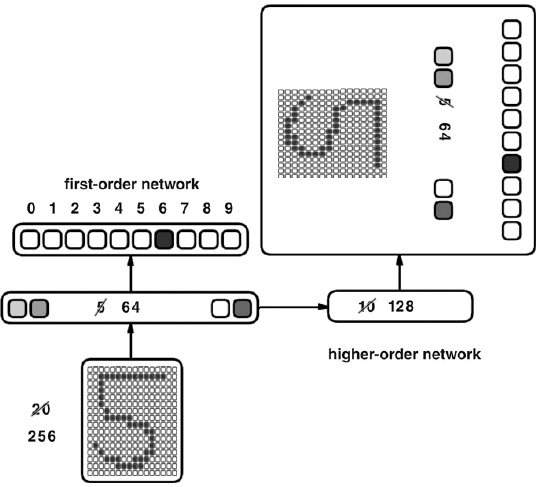
\includegraphics[width=130px]{../cleeremans_2007/digit_reco/schema_handwritten.png}
   &
   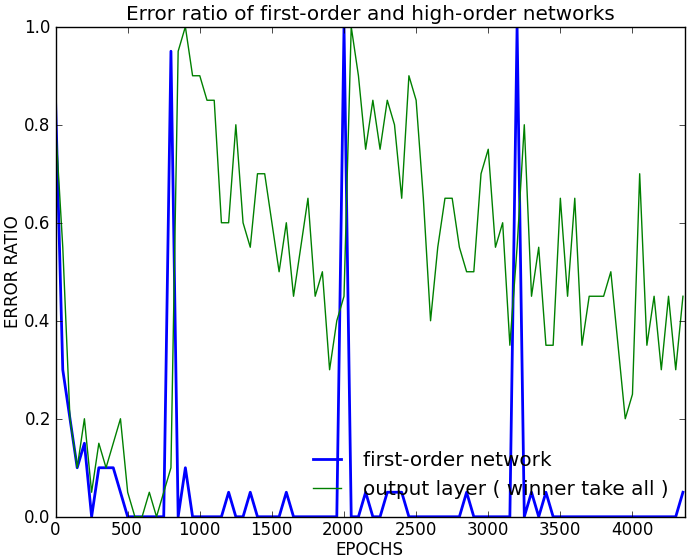
\includegraphics[width=190px]{../cleeremans_2007/digit_reco/err_handwritten_relearn_2.png}
  \end{tabular}
  \end{center}
\end{frame}


% ----------------------------------------------------------------------------------------------------
% ----------------------------------------------------------------------------------------------------
% ----------------------------------------------------------------------------------------------------


\begin{frame}
\tableofcontents[hideallsubsections]
\end{frame}


\section{Amélioration de l'apprentissage}

\begin{frame}
  \frametitle{La base de départ / Rappel}
  \begin{center}
    \begin{pspicture}(0,5)
      \rput[B](0,0){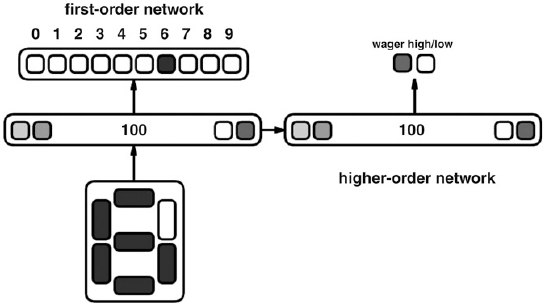
\includegraphics[height=150px]{../cleeremans_2007/digital_reco/schema.png}}
      \rput[B](3,0.5){\tiny{Consciousness and metarepresentation : A computational sketch}}
    \end{pspicture}
  \end{center}

  \begin{center}
    \begin{tabular}{lr}
    \begin{minipage}{150px}
      
      \footnotesize\begin{minusitemize}
      \item 7 entrées (afficheur digital)
      \item le premier réseau discrime les 10 chiffres
      \item winner-take-all sur les sorties
      \end{minusitemize}

      \end{minipage}
      &
      \begin{minipage}{170px}
      \footnotesize\begin{noitemize}
      \item la couche cachée du premier réseau sert d'entrée au second
      \item le second réseau apprend à parier sur la qualité de la réponse du premier
      \end{noitemize}
      
    \end{minipage}
    \end{tabular}
  \end{center}
  
\end{frame}



\begin{frame}
  \frametitle{Résultat sur la base d'entrée de l'article}
  \begin{center}
  Performances de classification
  \begin{tabular}{cc}
  \hspace*{-1cm}
   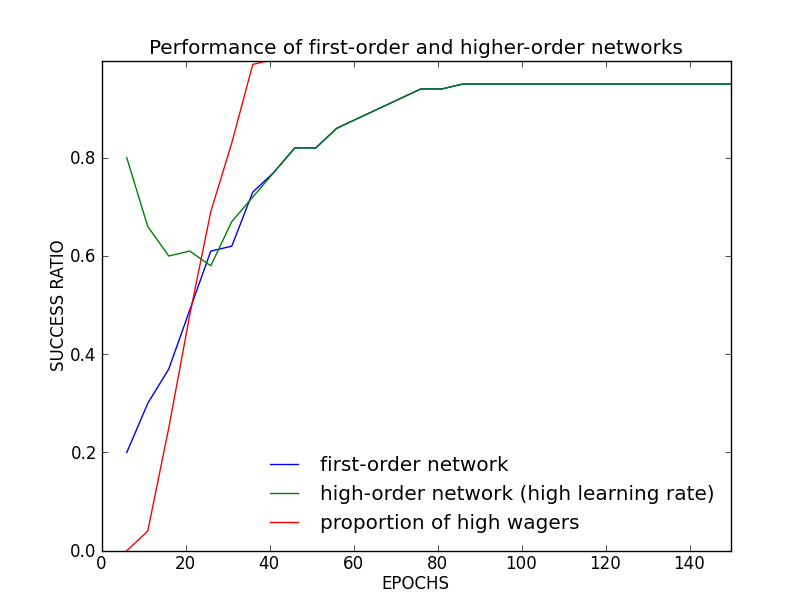
\includegraphics[width=175px]{../cleeremans_2007/digital_reco/perf_wag.png}
   &
   \hspace*{-0.3cm}
   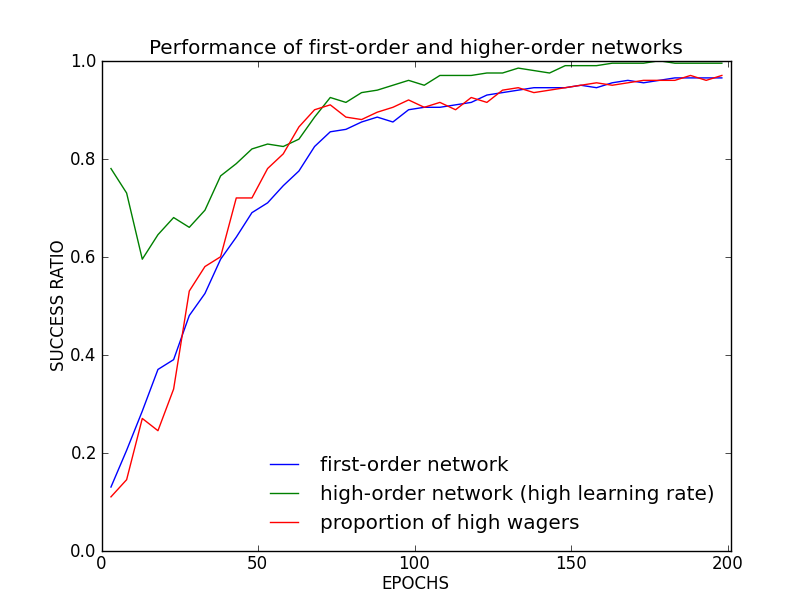
\includegraphics[width=175px]{../cleeremans_2007/digital_reco/perf_boost.png}
  \end{tabular}

  \begin{tabular}{lr}
  \begin{minipage}{170px}
    \hspace*{-0.2cm}
    \footnotesize Paramètre du second réseau :
    \footnotesize
      \begin{minusitemize}
      \item poids initilisés sur [-0.25; 0.25]
      \item momentum : 0
      \item non exploitable
      \end{minusitemize}
    \end{minipage}
    &
    \begin{minipage}{170px}
    \hspace*{0.2cm}
    \footnotesize Paramètre du second réseau :
    \footnotesize\begin{noitemize}
     \item poids initilisés sur [-1; 1]
     \item momentum : 0.5
     \item exploitable
    \end{noitemize}
    
    \end{minipage}
  \end{tabular}
  \end{center}
\end{frame}




\begin{frame}
  \frametitle{Passage à niveau}
  \begin{center}
  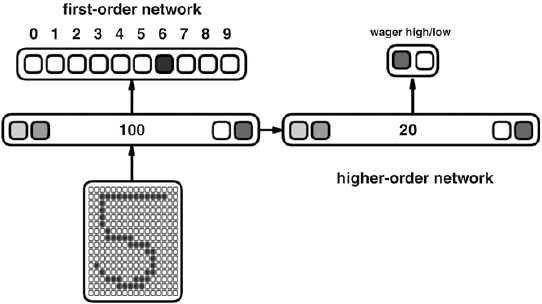
\includegraphics[height=150px]{base.png}
  \end{center}

  \begin{center}
  \begin{tabular}{lr}
  \begin{minipage}{150px}
    
    \footnotesize\begin{minusitemize}
     \item chiffres manuscrits sur 256 neurones d'entrées
     \item Le premier réseau discrime 1600 chiffres
     \item Winner-take-all sur les sorties
    \end{minusitemize}

    \end{minipage}
    &
    \begin{minipage}{170px}
    \footnotesize\begin{noitemize}
     \item la couche cachée du premier réseau sert d'entrée au second
     \item le second réseau apprend à parier sur la qualité de la réponse du premier
    \end{noitemize}
    
    \end{minipage}
  \end{tabular}

  \end{center}
  
\end{frame}



\begin{frame}
  \frametitle{Architectures de feedback}

  \hspace*{-0.8cm}
  \begin{tabular}{c|c|c}
  \begin{minipage}[b]{.33\linewidth}
   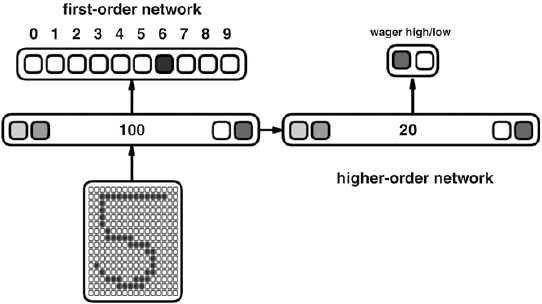
\includegraphics[width=100px]{base.png}
   \\
   \tiny Second neurone le plus élevé quand pari bas
   \end{minipage}
   
   &
   \begin{minipage}[b]{.33\linewidth}
      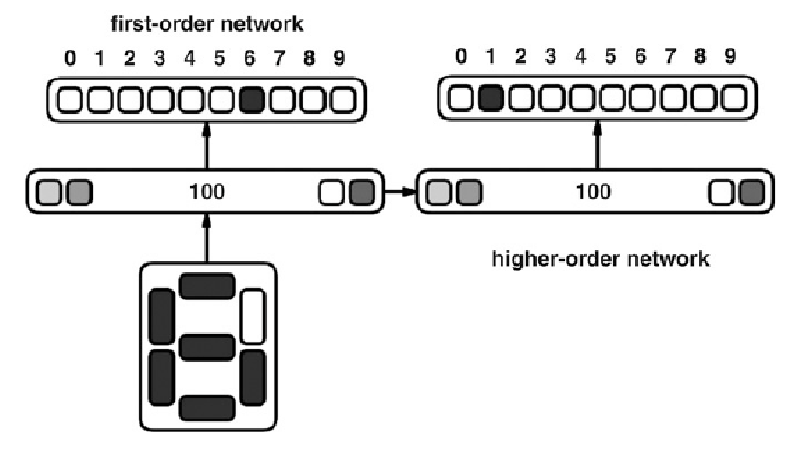
\includegraphics[width=100px]{../pre-presentation/nth_wta.png}
      \\
   \tiny Second réseau enregistre l'indice (par activation) du neurone contenant la bonne réponse
    \end{minipage}
   &
   \begin{minipage}[b]{.33\linewidth}
         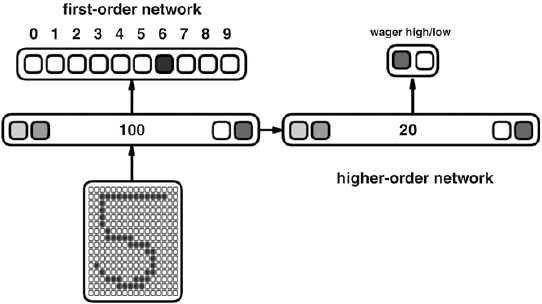
\includegraphics[width=100px]{base.png}
      \\
   \tiny Second réseau contrôle le taux d'apprentissage et le momentum du premier réseau
    \end{minipage}
    \\
    \hline
       \begin{minipage}[b]{.33\linewidth}
         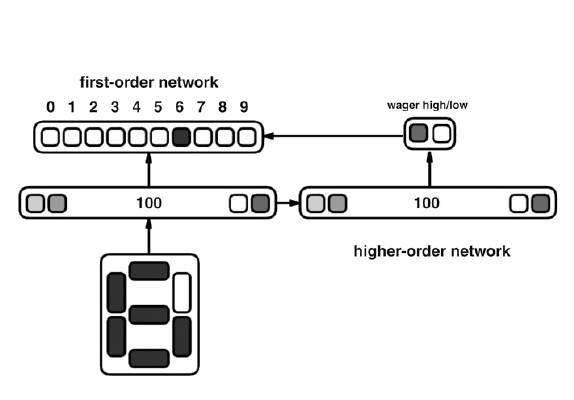
\includegraphics[width=100px]{../pre-presentation/merging.png}
      \\
   \tiny Les sorties du second réseaux deviennent des entrées supplémentaires au premier
    \end{minipage}
    &
    \begin{minipage}[b]{.33\linewidth}
         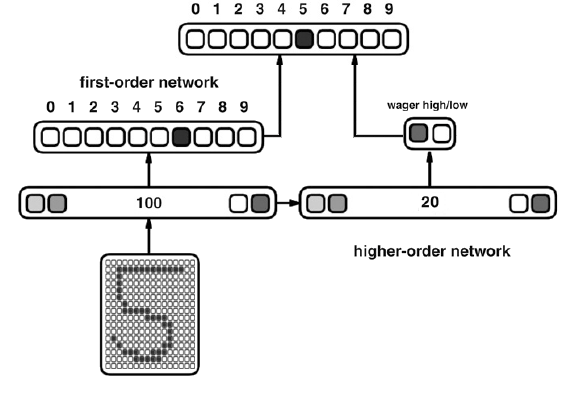
\includegraphics[width=100px]{../pre-presentation/thrid.png}
      \\
    \tiny 3ème réseau de perceptron
    \end{minipage}
    &
        \begin{minipage}[b]{.33\linewidth}
         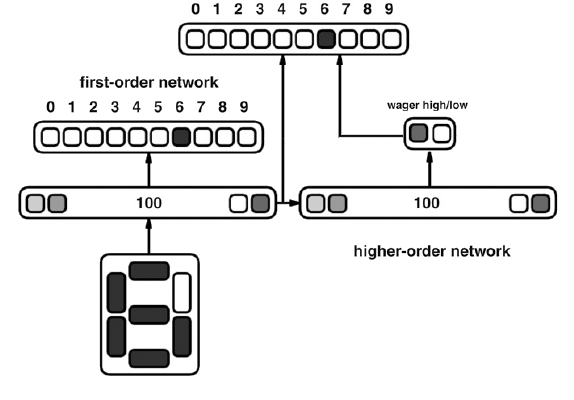
\includegraphics[width=100px]{../pre-presentation/thrid_hidden.png}
      \\
    \tiny 3ème réseau de perceptron sur la couche cachée
    \end{minipage}

  \end{tabular}


\end{frame}


\begin{frame}
  \frametitle{Résultat concluants}
  \framesubtitle{3ème réseau de perceptron}
  
  \begin{tabular}{cc}
  \hspace*{-1cm}
   
   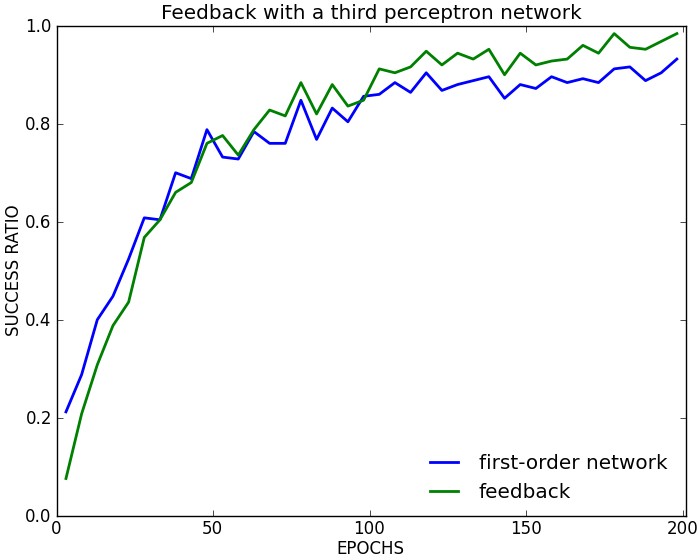
\includegraphics[width=175px]{../pre-rapport/third_net.png}
   &
   \hspace*{-0.3cm}
   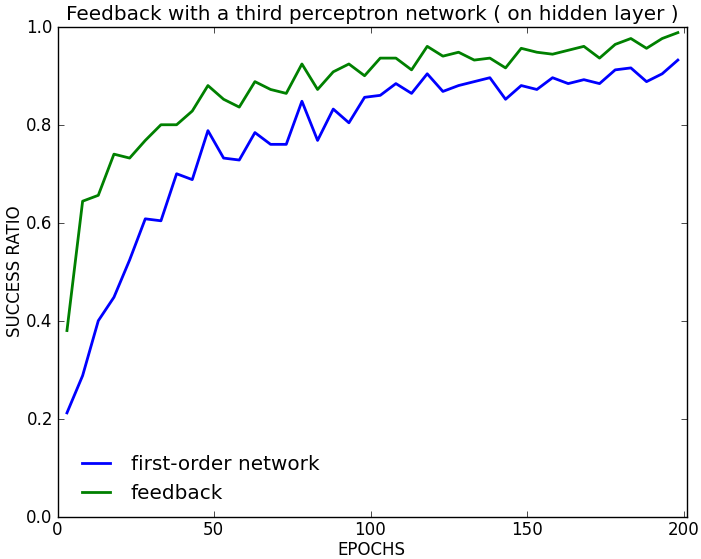
\includegraphics[width=175px]{../pre-rapport/third_net_hidden.png}
  \end{tabular}  
\end{frame}


\begin{frame}
  \frametitle{Limitations}
  Le nombre de neurone dans la couche cachée du FoN déterminent beaucoup les performances :
  \begin{itemize}
   \item si il est ``normal'', le second réseau n'arrivera pas à parier efficacement, et se contente de 
   parier haut
   \item si il est élevé, le second réseau parie correctement, mais le premier réseau est détérioré.
   \newline
   De sorte que même avec l'augmentation de performance du SoN, il ne dépasse pas un FoN bien réglé
  \end{itemize}

\end{frame}

\begin{frame}
  \frametitle{Limitations}
  \begin{center}
    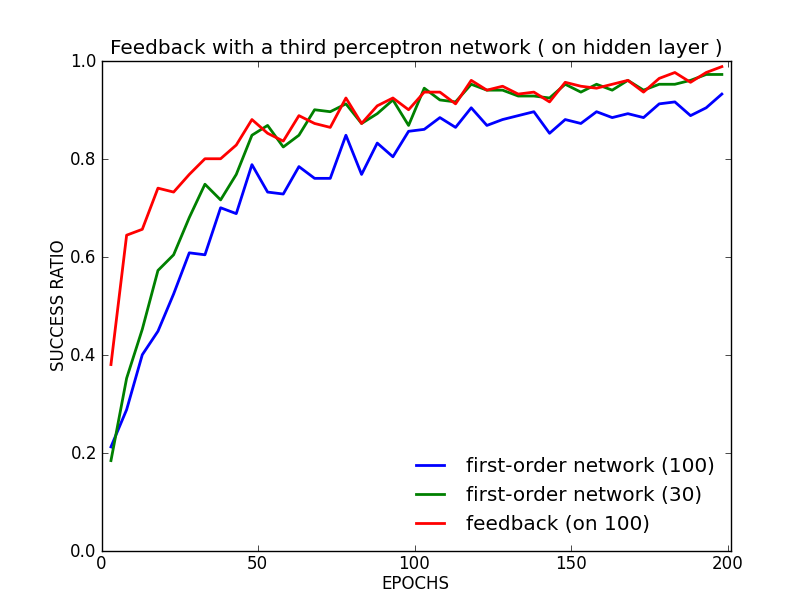
\includegraphics[height=220px]{../cleeremans_2007/digit_reco/bad_full.png}
  \end{center}
\end{frame}

% \begin{frame}
%   \frametitle{Conclusion}
%  En performances
%  
%  En terme d'interprétation
% \end{frame}




% \section{Transfert de tâche}
% \begin{frame}
% 
% \end{frame}
% 
% \begin{frame}
% 
% \end{frame}
% \section{Conscience}
% \begin{frame}
% 
% \end{frame}






% 
% 
% --------------------------------------------------------------------------------------------
% --------------------------------------------------------------------------------------------
% --------------------------------------------------------------------------------------------
% --------------------------------------------------------------------------------------------
% --------------------------------------------------------------------------------------------
% \section[Sujet 1 : Jeu vidéo]{Sujet 1 : Jeu vidéo}
% 
% % \subsection[titre cour2t1]{titre long long long 1}
% 
% 
% \subsection[ ]{ }
% \begin{frame}
%  \frametitle{Sujet 1 : Jeu vidéo C++ en pseudo-3D (isométrique)}
%  \framesubtitle{Introduction}
%   \begin{itemize}[<+->]
%     \item Difficulté : de 3 à 4 étoiles
%       \begin{itemize}[<+->]
% \item C++ ( pointeurs, références, mémoire, templates, règles, ...)
% \item Bibliotèques : Boost / CEGUI / SFML
% \item Algorithmes : collision, pathfinding, affichage, IA, déplacement, ...
% \item Portalibité
% \item Durée \& Graphisme
% \item Echanges client/serveur
%       \end{itemize}
%     \item Durée : de 3 à 5 étoiles
%     \item Langages
%       \begin{itemize}[<+->]
% \item C++
% \item OpenGL
% \item Lua
% \item XML
% \item PostgreSQL
%       \end{itemize}
%   \end{itemize}
% \end{frame}
% 
% 
% \begin{frame}
%  \frametitle{Sujet 1 : Jeu vidéo C++ en pseudo-3D (isométrique)}
%  \framesubtitle{Jeu 2D}
%  \begin{center}
%   \includegraphics[height=200px]{data/2D_1.jpg}
%  \end{center}
% \end{frame}
% 
% \begin{frame}
%  \frametitle{Sujet 1 : Jeu vidéo C++ en pseudo-3D (isométrique)}
%  \framesubtitle{Jeu 3D}
%  \begin{center}
%   \includegraphics[height=200px]{data/3D_1.jpg}
%  \end{center}
% \end{frame}
% 
% 
% \begin{frame}
%  \frametitle{Sujet 1 : Jeu vidéo C++ en pseudo-3D (isométrique)}
%  \framesubtitle{Perspective Isométrique}
%  \includegraphics[height=196px]{data/wakfu_screen3.jpg}
% \end{frame}
% 
% \begin{frame}
%  \frametitle{Sujet 1 : Jeu vidéo C++ en pseudo-3D (isométrique)}
%  \framesubtitle{SFML vs CEGUI}
%  \includegraphics[height=196px]{data/wakfu_screen3.jpg}
% \end{frame}
% 
% \begin{frame}
%  \frametitle{Sujet 1 : Jeu vidéo C++ en pseudo-3D (isométrique)}
%  \framesubtitle{Découpage}
%  \begin{center}
%  \includegraphics[height=196px]{data/S1_decoup.png}
%   \end{center}
% \end{frame}
% 
% \begin{frame}
%  \frametitle{Sujet 1 : Jeu vidéo C++ en pseudo-3D (isométrique)}
%  \framesubtitle{Intérêts}
%   \begin{itemize}[<+->]
%     \item Prise en main d'un moteur graphique avancé (SFML)
%     \item Prise en main d'une GUI avancée (CEGUI)
%     \item Compréhension des mécanismes d'échanges entre GUI-moteur graphique
%     \item Découverte d'architectures pour jeux-vidéos
%     \item Mise en place de protocoles de communication personnalisés ( si serveur )
%     \item Equipe pluridisciplinaire (graphistes, scénaristes, ingé. son, ...)
%     \item Beaucoup d'autres choses dépendant du type de jeu choisi
%   \end{itemize}
% \end{frame}
% 
% \begin{frame}
%  \frametitle{Sujet 1 : Jeu vidéo C++ en pseudo-3D (isométrique)}
%  \framesubtitle{Conclusion}
%   \begin{itemize}[<+->]
%     \item Très enrichissant
%     \item Possibilitées de financement ( publicité, F2P, services, ... )
%     \item Long et dépendant d'autrui
%     \item \bf{Originalité}
%   \end{itemize}
%   
%    \uncover<5->{
%     \begin{block}{ Chances de réussite }
% 60\%
%     \end{block}
%    }
%    
% \end{frame}
% 
% \section[Sujet 2 : IHM]{Sujet 2 : IHM}
% 
% \subsection[ ]{ }
% \begin{frame}
%  \frametitle{Sujet 2 : IHM (interface homme-machine) virtuelle}
%  \framesubtitle{Introduction}
%   \begin{itemize}[<+->]
%     \item Difficulté : de 3 à 5 étoiles
%       \begin{itemize}[<+->]
% \item Algorithmes avancés d'I.A ( réseaux de neurones, réseau bayésien, chaîne de Markov cachées, ... )
% \item Pas toujours au point
% \item Pas toujours libre
% \item Travail de recherche ( lire articles , ... )
%       \end{itemize}
%     \item Durée : de 2 à 5 étoiles
%     \item Langages : ?
%   \end{itemize}
% \end{frame}
% 
% \begin{frame}
%  \frametitle{Sujet 2 : IHM (interface homme-machine) virtuelle}
%  \framesubtitle{C'est quoi?}
%  \begin{center}
%  \includegraphics[height=196px]{data/holo.jpg}
%   \end{center}
% \end{frame}
% 
% \begin{frame}
%  \frametitle{Sujet 2 : IHM (interface homme-machine) virtuelle}
%  \framesubtitle{Structure}
%  \begin{center}
%  \includegraphics[height=196px]{data/S2_schema.jpg}
%   \end{center}
% \end{frame}
% 
% \begin{frame}
%  \frametitle{Sujet 2 : IHM (interface homme-machine) virtuelle}
%  \framesubtitle{Intérêts}
%  \begin{center}
%  \includegraphics[height=130px]{data/S2_schema.jpg}
%   \end{center}
%     \begin{itemize}
%       \item<2-> intéractions avec ordinateur ( musique, recherche, ...)
%       \item<3-> intéractions avec monde réel ( contrôle maison, ...)
%     \end{itemize}
% \end{frame}
% 
% \begin{frame}
%  \frametitle{Sujet 2 : IHM (interface homme-machine) virtuelle}
%  \framesubtitle{Conclusion}
%   \begin{itemize}[<+->]
%     \item Très enrichissant au niveau de l'IA
%     \item Bonne introduction à la recherche
%     \item Peu de possibilitées de financement ( publicité, vente logiciel, ... )
%     \item Long, compliqué
%     \item \bf{Incomplet / Imparfait}
%   \end{itemize}
%   
%    \uncover<6->{
%     \begin{alertblock}{ Chances de réussite }
% 20\%
%     \end{alertblock}
%    }
%    
% \end{frame}
% 
% 
% \section[Sujet 3 : Serveur]{Sujet 3 : Serveur}
% 
% \subsection[ ]{ }
% \begin{frame}
%  \frametitle{Sujet 3 : Vulgarisation de serveur (+décentralisation)}
%  \framesubtitle{Introduction}
%   \begin{itemize}[<+->]
%     \item Difficulté : 2 étoiles
%       \begin{itemize}[<+->]
% \item Savoir configurer les différents outils
% \item Transactions sécurisées
%       \end{itemize}
%     \item Durée : de 2 à 4 étoiles
%     \item Langages : JSE/JEE/C
%       \begin{itemize}[<+->]
% \item Bash
%       \end{itemize}
%   \end{itemize}
% \end{frame}
% 
% \begin{frame}
%  \frametitle{Sujet 3 : Vulgarisation de serveur (+décentralisation)}
%  \framesubtitle{Structure}
%  \begin{center}
%   \includegraphics[height=196px]{data/S3_schema.jpg}
%  \end{center}
% \end{frame}
% 
% \begin{frame}
%  \frametitle{Sujet 3 : Vulgarisation de serveur (+décentralisation)}
%  \framesubtitle{Aller plus loin}
%  Décentraliser les services
%  \begin{itemize}
%   \item<2-> Chat
%   \item<3-> Streaming
%   \item<4-> ...
%  \end{itemize}
% 
% \end{frame}
% 
% 
% \begin{frame}
%  \frametitle{Sujet 3 : Vulgarisation de serveur (+décentralisation)}
%  \framesubtitle{Conclusion}
%   \begin{itemize}[<+->]
%     \item Peu enrichissant au niveau de l'algorithmique
%     \item Enrichissant sur les différents outils
%     \item Pas de possibilitées de financement
%     \item Peut être soutenu par une communauté libre
%     \item \bf{Motivation}
%   \end{itemize}
%   
%    \uncover<6->{
%     \begin{exampleblock}{ Chances de réussite }
% 75\%
%     \end{exampleblock}
%    }
%    
% \end{frame}
% 
% \section[Sujet 4 : Dialogues]{Sujet 4 : Dialogues}
% 
% \subsection[ ]{ }
% \begin{frame}
%  \frametitle{Sujet 4 : Dialogues non instantanés par prévisions}
%  \framesubtitle{Introduction}
%   \begin{itemize}[<+->]
%     \item Difficulté : de 1 étoiles
%       \begin{itemize}[<+->]
% \item Mélange dot et javascript
%       \end{itemize}
%     \item Durée : de 1 étoile
%     \item Langages :
%       \begin{itemize}
%      \item Java ( JSF / JPA / ... )
%      \item Javascript ( Jquery / ... )
%       \end{itemize}
%   \end{itemize}
% \end{frame}
% 
% 
% \begin{frame}
%  \frametitle{Sujet 4 : Dialogues non instantanés par prévisions}
%  \framesubtitle{Structure}
%  \begin{center}
%   \includegraphics[height=190px]{data/S4_schema.jpg}
%  \end{center}
% \end{frame}
% 
% 
% \begin{frame}
%  \frametitle{Sujet 4 : Dialogues non instantanés par prévisions}
%  \framesubtitle{Conclusion}
%   \begin{itemize}[<+->]
%     \item Très peu enrichissant
%     \item Possibilitées de financement ( publicité, services, ... )
%     \item Financements faibles
%     \item \bf{Facilité}
%   \end{itemize}
%   
%    \uncover<5->{
%     \begin{exampleblock}{ Chances de réussite }
% 90\%
%     \end{exampleblock}
%    }
%    
% \end{frame}
% 
% 
% \section[Récapitulatif]{Récapitulatif}
% 
% \subsection[ ]{ }
% \begin{frame}
%  \frametitle{Différences}
%  \begin{center}
%   \begin{tabular}{|l|c|c|c|}
%   \hline
%   Sujets & Intéressant & Financements & Réussite \\
%   \hline
%   Sujet 1 : Jeu vidéo & 3.5 & 4 & 60\%
%   \\
%   \hline
%   Sujet 2 : IHM & 4 & 1 & 20\%
%   \\
%   \hline
%   Sujet 3 : Serveur & 2 & 0 & 75\%
%   \\
%   \hline
%   Sujet 4 : Dialogues & 1 & 3 & 90\%
%   \\
%   \hline
%   \end{tabular}
%  \end{center}
% \end{frame}

\end{document}


